%%%
 %
 % Copyright (C) 2020 Ángel Iván Gladín García
 %
 % This program is free software: you can redistribute it and/or modify
 % it under the terms of the GNU General Public License as published by
 % the Free Software Foundation, either version 3 of the License, or
 % (at your option) any later version.
 %
 % This program is distributed in the hope that it will be useful,
 % but WITHOUT ANY WARRANTY; without even the implied warranty of
 % MERCHANTABILITY or FITNESS FOR A PARTICULAR PURPOSE.  See the
 % GNU General Public License for more details.
 %
 % You should have received a copy of the GNU General Public License
 % along with this program.  If not, see <http://www.gnu.org/licenses/>.
%%%

%%%%%%%%%%%%%%%%%%%%%%%%%%%%%%%%%%%%%%%%%%%%%%%%%%%%%%%%%%%%%%%%%%%%%%%%%%%%%%%%%%%%%%%%%
\documentclass{article}

\usepackage{tikz}
\usetikzlibrary{arrows,automata,positioning, calc}
\tikzset{node distance=2.5cm, % Minimum distance between two nodes. Change if necessary.
        every state/.style={ % Sets the properties for each state
            semithick,
            fill=gray!10},
        initial text={}, % No label on start arrow
        double distance=2pt, % Adjust appearance of accept states
        every edge/.style={ % Sets the properties for each transition
            draw,
            ->,>=stealth', % Makes edges directed with bold arrowheads
            auto,
            semithick}
        }
\let\epsilon\varepsilon
\usepackage[utf8]{inputenc}


\begin{document}

%%%%%%%%

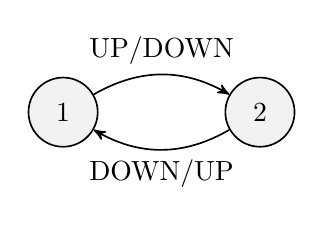
\begin{tikzpicture}
    \node[state] (1) {1};
    \node[state, right of=1] (2) {2};

    \draw (1) edge[bend left] node {UP/DOWN} (2);
    \draw (2) edge[bend left] node {DOWN/UP} (1);
\end{tikzpicture}

%%%%%%%%

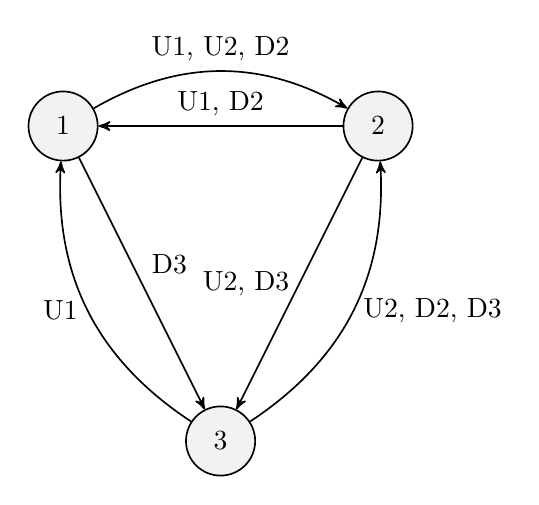
\begin{tikzpicture}
    \node[state] (1) at (0,4) {1};
    \node[state] (2) at (4,4) {2};
    \node[state] (3) at (2,0) {3};

    \draw (1) edge[bend left] node[above] {U1, U2, D2} (2);
    \draw (3) edge[bend right] node[right] {U2, D2, D3} (2);
    \draw (3) edge[bend left] node[left] {U1} (1);
    
    \draw (2) edge node[above] {U1, D2} (1);
    \draw (1) edge node {D3} (3);
    \draw (2) edge node[above, left] {U2, D3} (3);
\end{tikzpicture}

%%%%%%%%

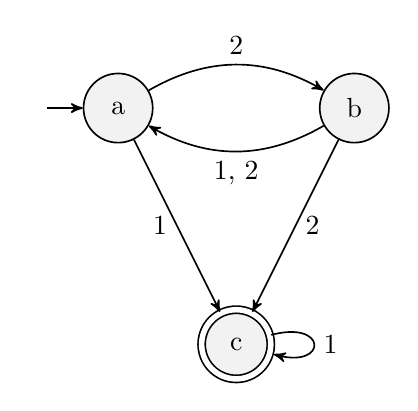
\begin{tikzpicture}
    \node[state, initial]   (a) at (0,3)   {a};
    \node[state]            (b) at (3,3)   {b};
    \node[state, accepting] (c) at (1.5,0) {c};

    \draw (a) edge[bend left] node[above] {2}    (b);
    \draw (b) edge[bend left] node[below] {1, 2} (a);
    
    \draw (a) edge node[left]  {1} (c);
    \draw (b) edge node[right] {2} (c);

    \draw (c) edge[loop right] node {1} (c);
\end{tikzpicture}

%%%%%%%%

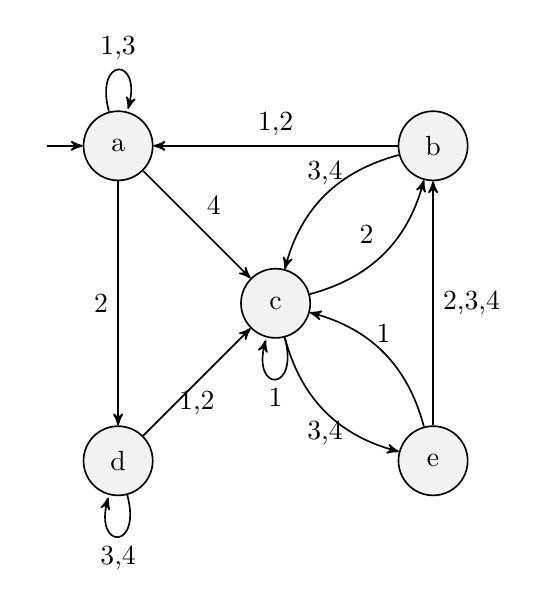
\begin{tikzpicture}
    \node[state, initial] (a) at (0,4) {a};
    \node[state] (b) at (4,4) {b};
    \node[state] (c) at (2,2) {c};
    \node[state] (d) at (0,0) {d};
    \node[state] (e) at (4,0) {e};

    \draw (a) edge node[left] {2} (d);
    \draw (b) edge node[above] {1,2} (a);
    \draw (e) edge node[right] {2,3,4} (b);
    \draw (a) edge node {4} (c);
    \draw (d) edge node[below] {1,2} (c);

    \draw (b) edge[bend right] node[above] {3,4} (c);
    \draw (c) edge[bend right] node {2} (b);
    \draw (e) edge[bend right] node[above] {1} (c);
    \draw (c) edge[bend right] node[below] {3,4} (e);

    \draw (a) edge[loop above] node {1,3} (a);
    \draw (d) edge[loop below] node {3,4} (d);
    \draw (c) edge[loop below] node {1} (c);
\end{tikzpicture}

%%%%%%%%

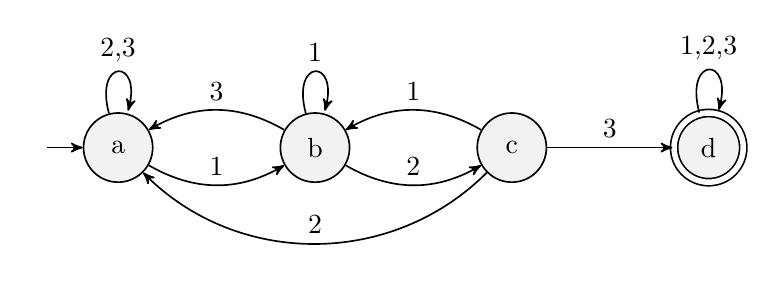
\begin{tikzpicture}
    \node[state,initial]    (a)                 {a};
    \node[state]            (b)  [right of=a]   {b};
    \node[state]            (c)  [right of=b]   {c};
    \node[state,accepting]  (d)  [right of=c]   {d};

    \draw (c) edge node {3} (d);

    \draw (a) edge [bend right] node {1} (b);
    \draw (b) edge [bend right] node[above] {3} (a);
    \draw (c) edge [bend right] node[above] {1} (b);
    \draw (b) edge [bend right] node {2} (c);
    \draw (c) edge [bend left=45] node[above] {2} (a);

    \draw (a) edge[loop above] node {2,3} (a);
    \draw (b) edge[loop above] node {1} (b);
    \draw (d) edge[loop above] node {1,2,3} (d);
\end{tikzpicture}

%%%%%%%%
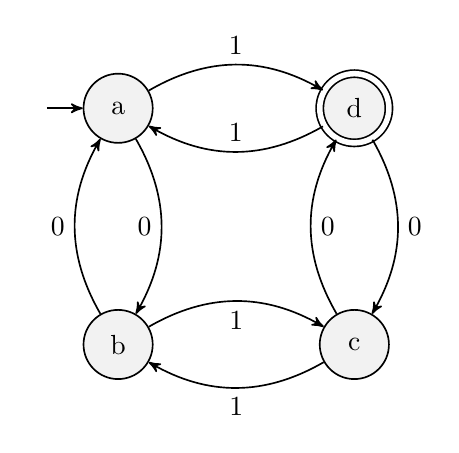
\begin{tikzpicture}
    \node[state,initial]   (a) at (0,3) {a};
    \node[state,accepting] (d) at (3,3) {d};
    \node[state]           (b) at (0,0) {b};
    \node[state]           (c) at (3,0) {c};

    \draw
        (a)
            edge[bend left] node[left]  {0} (b)
            edge[bend left] node[above] {1} (d)
        (b)
            edge[bend left] node[below] {1} (c)
            edge[bend left] node[left]  {0} (a)
        (c)
            edge[bend left] node[below] {1} (b)
            edge[bend left] node[right] {0} (d)
        (d)
            edge[bend left] node[above] {1} (a)
            edge[bend left] node[right] {0} (c);
\end{tikzpicture}
%%%%%%%%

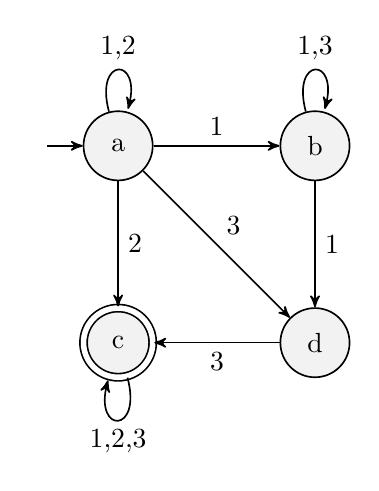
\begin{tikzpicture}
    \node[state,initial]    (a)                 {a};
    \node[state]            (b) [right of=a]    {b};
    \node[state,accepting]  (c) [below of=a]    {c};
    \node[state]            (d) [below of=b]    {d};

    \draw
        (a)
            edge [loop above] node {1,2}    ()
            edge node {1} (b)
            edge node {2} (c)
            edge node {3} (d)
        (b)
            edge [loop above] node {1,3}    ()
            edge node {1} (d)
        (c)
            edge [loop below] node {1,2,3} ()
        (d)
            edge [below] node {3} (c);
\end{tikzpicture}

%%%%%%%%

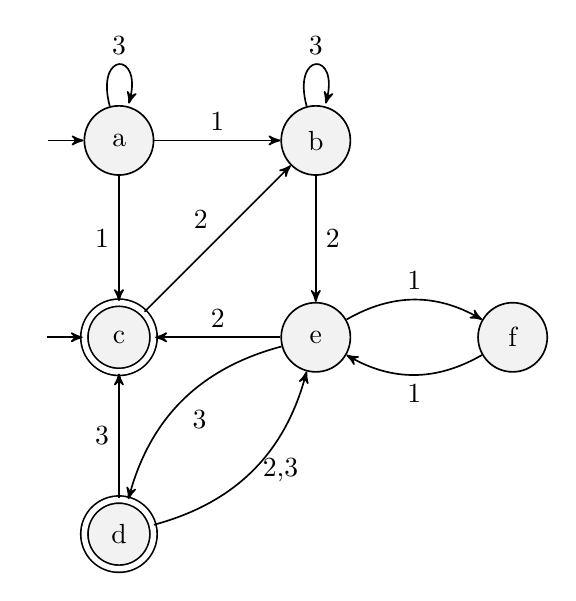
\begin{tikzpicture}
    \node[state, initial] (a) {a};
    \node[state] (b) [right of=a] {b};
    \node[state, initial, accepting] (c) [below of=a] {c};
    \node[state] (e) [right of=c] {e};
    \node[state] (f) [right of=e] {f};
    \node[state, accepting] (d) [below of=c] {d};

    \draw
        (a)
            edge [loop above] node {3} ()
            edge node {1} (b)
            edge node [left] {1} (c)
        (b)
            edge [loop above] node {3} ()
            edge node {2} (e)
        (c)
            edge node {2} (b)
        (d)
            edge node {3} (c)
            edge [bend right] node [right] {2,3} (e)
        (e)
            edge node [above] {2} (c)
            edge [bend right] node {3} (d)
            edge [bend left] node {1} (f)
        (f)
            edge [bend left] node {1} (e);
\end{tikzpicture}

%%%%%%%%
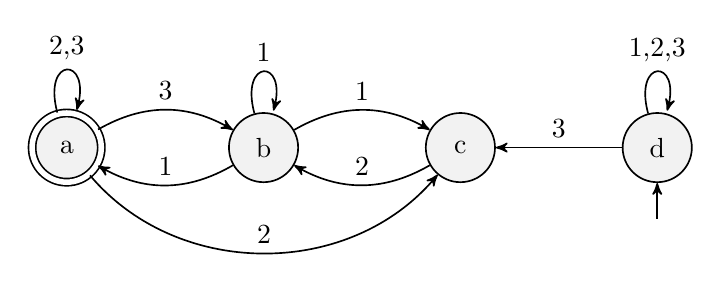
\begin{tikzpicture}
    \node[state, accepting] (a) {a};
    \node[state] (b) [right of =a] {b};
    \node[state] (c) [right of =b] {c};
    \node[state, initial below] (d) [right of =c] {d};

    \draw
        (a)
            edge [loop above] node {2,3} ( )
            edge [bend left] node {3} (b)
            edge [bend right=50] node {2} (c)
        (b)
            edge [loop above] node {1} ( )
            edge [bend left] node [above] {1} (a)
            edge [bend left] node {1} (c)
        (c)
            edge [bend left] node [above] {2} (b)
        (d)
            edge [loop above] node {1,2,3} ( )
            edge node [above] {3} (c);
\end{tikzpicture}

%%%%%%%%
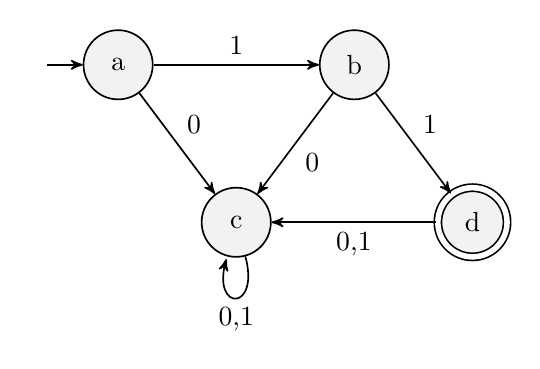
\begin{tikzpicture}
    \node[state,initial]   (a) at (0,2) {a};
    \node[state] (b) at (3,2) {b};
    \node[state]           (c) at (1.5,0) {c};
    \node[state, accepting] (d) at (4.5,0) {d};

    \draw
        (a)
            edge node {1} (b)
            edge node {0} (c)
        (b)
            edge node {0} (c)
            edge node {1} (d)
        (c)
            edge [loop below] node {0,1} ( )
        (d)
            edge node {0,1} (c);
\end{tikzpicture}
%%%%%%%%

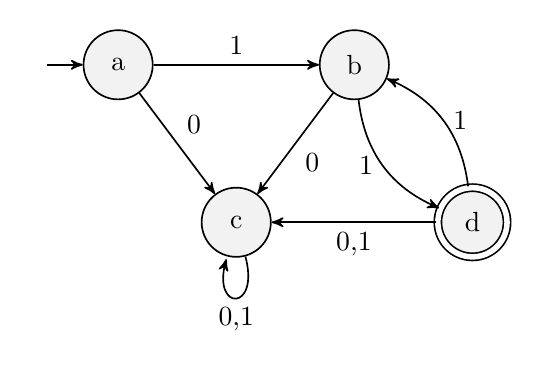
\begin{tikzpicture}
    \node[state,initial]   (a) at (0,2) {a};
    \node[state] (b) at (3,2) {b};
    \node[state]           (c) at (1.5,0) {c};
    \node[state, accepting] (d) at (4.5,0) {d};

    \draw
        (a)
            edge node {1} (b)
            edge node {0} (c)
        (b)
            edge node {0} (c)
            edge [bend right] node [left] {1} (d)
        (c)
            edge [loop below] node {0,1} ( )
        (d)
            edge [bend right] node [right] {1} (b)
            edge node {0,1} (c);
\end{tikzpicture}

%%%%%%%%
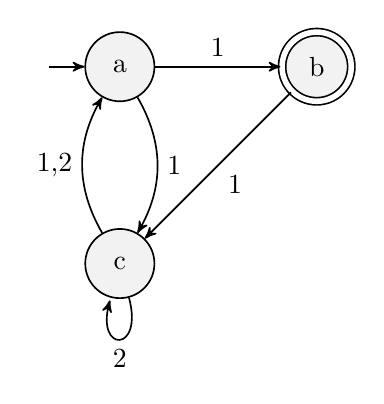
\begin{tikzpicture}
    \node[state,initial] (a) {a};
    \node[state, accepting] (b) [right of =a] {b};
    \node[state] (c) [below of =a] {c};

    \draw
        (a)
            edge node {1} (b)
            edge [bend left] node {1} (c)
        (b)
            edge node {1} (c)
        (c)
            edge [bend left] node {1,2} (a)
            edge [loop below] node {2} ( );
\end{tikzpicture}

%%%%%%%%

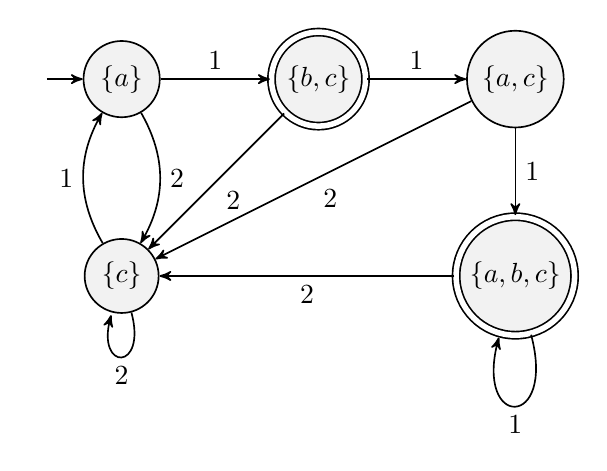
\begin{tikzpicture}
    \node[state,initial] (q1) {$\{ a \}$};
    \node[state, accepting] (q2) [right of=q1] {$\{ b,c \}$};
    \node[state] (q3) [right of =q2] {$\{ a,c \}$};
    \node[state] (q4) [below of =q1] {$\{ c \}$};
    \node[state, accepting] (q5) [below of =q3] {$\{ a,b,c \}$};

    \draw
        (q1)
            edge node {1} (q2)
            edge [bend left] node {2} (q4)
        (q2)
            edge node {1} (q3)
            edge node {2} (q4)
        (q3)
            edge node {2} (q4)
            edge node {1} (q5)
        (q4)
            edge [loop below] node {2} ( )
            edge [bend left] node {1} (q1)
        (q5)
            edge [loop below] node {1} ( )
            edge node {2} (q4);
\end{tikzpicture}

%%%%%%%%
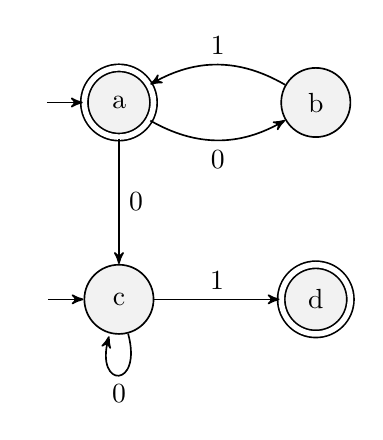
\begin{tikzpicture}
    \node[state, initial, accepting] (a) {a};
    \node[state] (b) [right of=a] {b};
    \node[state, initial] (c) [below of=a] {c};
    \node[state, accepting] (d) [right of=c] {d};

    \draw
        (a)
            edge [bend right] node [below] {0} (b)
            edge node {0} (c)
        (b)
            edge [bend right] node [above] {1} (a)
        (c)
            edge [loop below] node {0} ( )
            edge node {1} (d);
\end{tikzpicture}
%%%%%%%%

%%% TODO página 184 aristas, de aquí en adelante
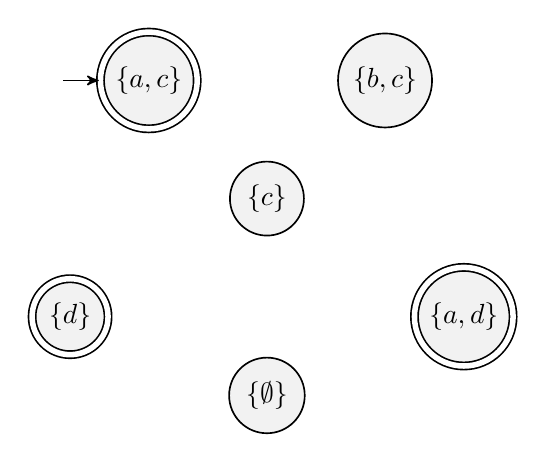
\begin{tikzpicture}
    \node[state, initial, accepting] (q1) at (1,4) {$\{ a,c \}$};
    \node[state] (q2) at (4,4) {$\{ b,c \}$};
    \node[state] (q3) at (2.5,2.5) {$\{ c \}$};
    \node[state, accepting] (q4) at (0,1) {$\{ d \}$};
    \node[state, accepting] (q5) at (5,1) {$\{ a,d \}$};
    \node[state] (q6) at (2.5,0) {$\{ \emptyset \}$};
\end{tikzpicture}
%%%%%%%%

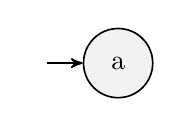
\begin{tikzpicture}
    \node[state, initial] (a) {a};
\end{tikzpicture}
%%%%%%%%

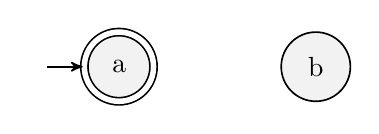
\begin{tikzpicture}
    \node[state, initial, accepting] (a) {a};
    \node[state] (b) [right of=a] {b};
\end{tikzpicture}

%%%%%%%%
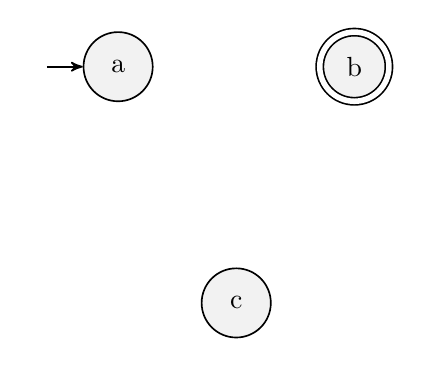
\begin{tikzpicture}
    \node[state, initial] (a) at (0,3) {a};
    \node[state, accepting] (b) at (3,3) {b};
    \node[state] (c) at (1.5,0) {c};
\end{tikzpicture}

%%%%%%%%
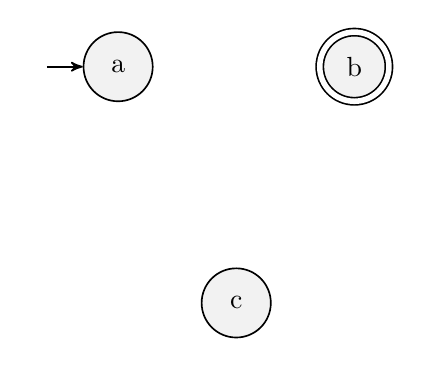
\begin{tikzpicture}
    \node[state, initial] (a) at (0,3) {a};
    \node[state, accepting] (b) at (3,3) {b};
    \node[state] (c) at (1.5,0) {c};
\end{tikzpicture}
%%%%%%%%

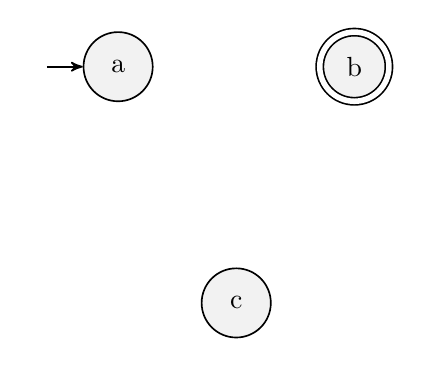
\begin{tikzpicture}
    \node[state, initial] (a) at (0,3) {a};
    \node[state, accepting] (b) at (3,3) {b};
    \node[state] (c) at (1.5,0) {c};
\end{tikzpicture}
%%%%%%%%

\end{document}
